

In this section I cross-validate the robustness of the initials results by re-estimating the models with altered variables in order to confirm that the appearance of over-performance is not created artificially. Thus, the practice can lead to validation or invalidation along with advancement of model specifications. 

For both the Market Model and the Calendar Time Portfolio I 1) alter the threshold for events to be considered as important from one to two and three standard deviations, and 2) change the portfolio weights from being based on market capitalization (value) to a naive approach (equal). Due to insignificance and borderline randomness of the relation between positive events and returns I only present the plots related to negative events. The comparable graphs of the positive events can be found in Appendix \ref{fig:ST_pos_sensi}.

\subsection{Market model: event threshold} \label{sec: sens_st_sd}

The requirements behind the thresholds for event identification is based on the volume of events relative to the average throughout the full sample for a given firm. Increasing the threshold naturally leads to fewer stocks included in the calculation of average abnormal returns. Intuitively, an increase in the tightness of the threshold is expected capture more extreme events, which should to lead to higher abnormal returns in absolute values, if firms with larger events are penalized harder.  

\begin{figure} [H]
    \centering
    \caption{Negative news: Update event requirement}
    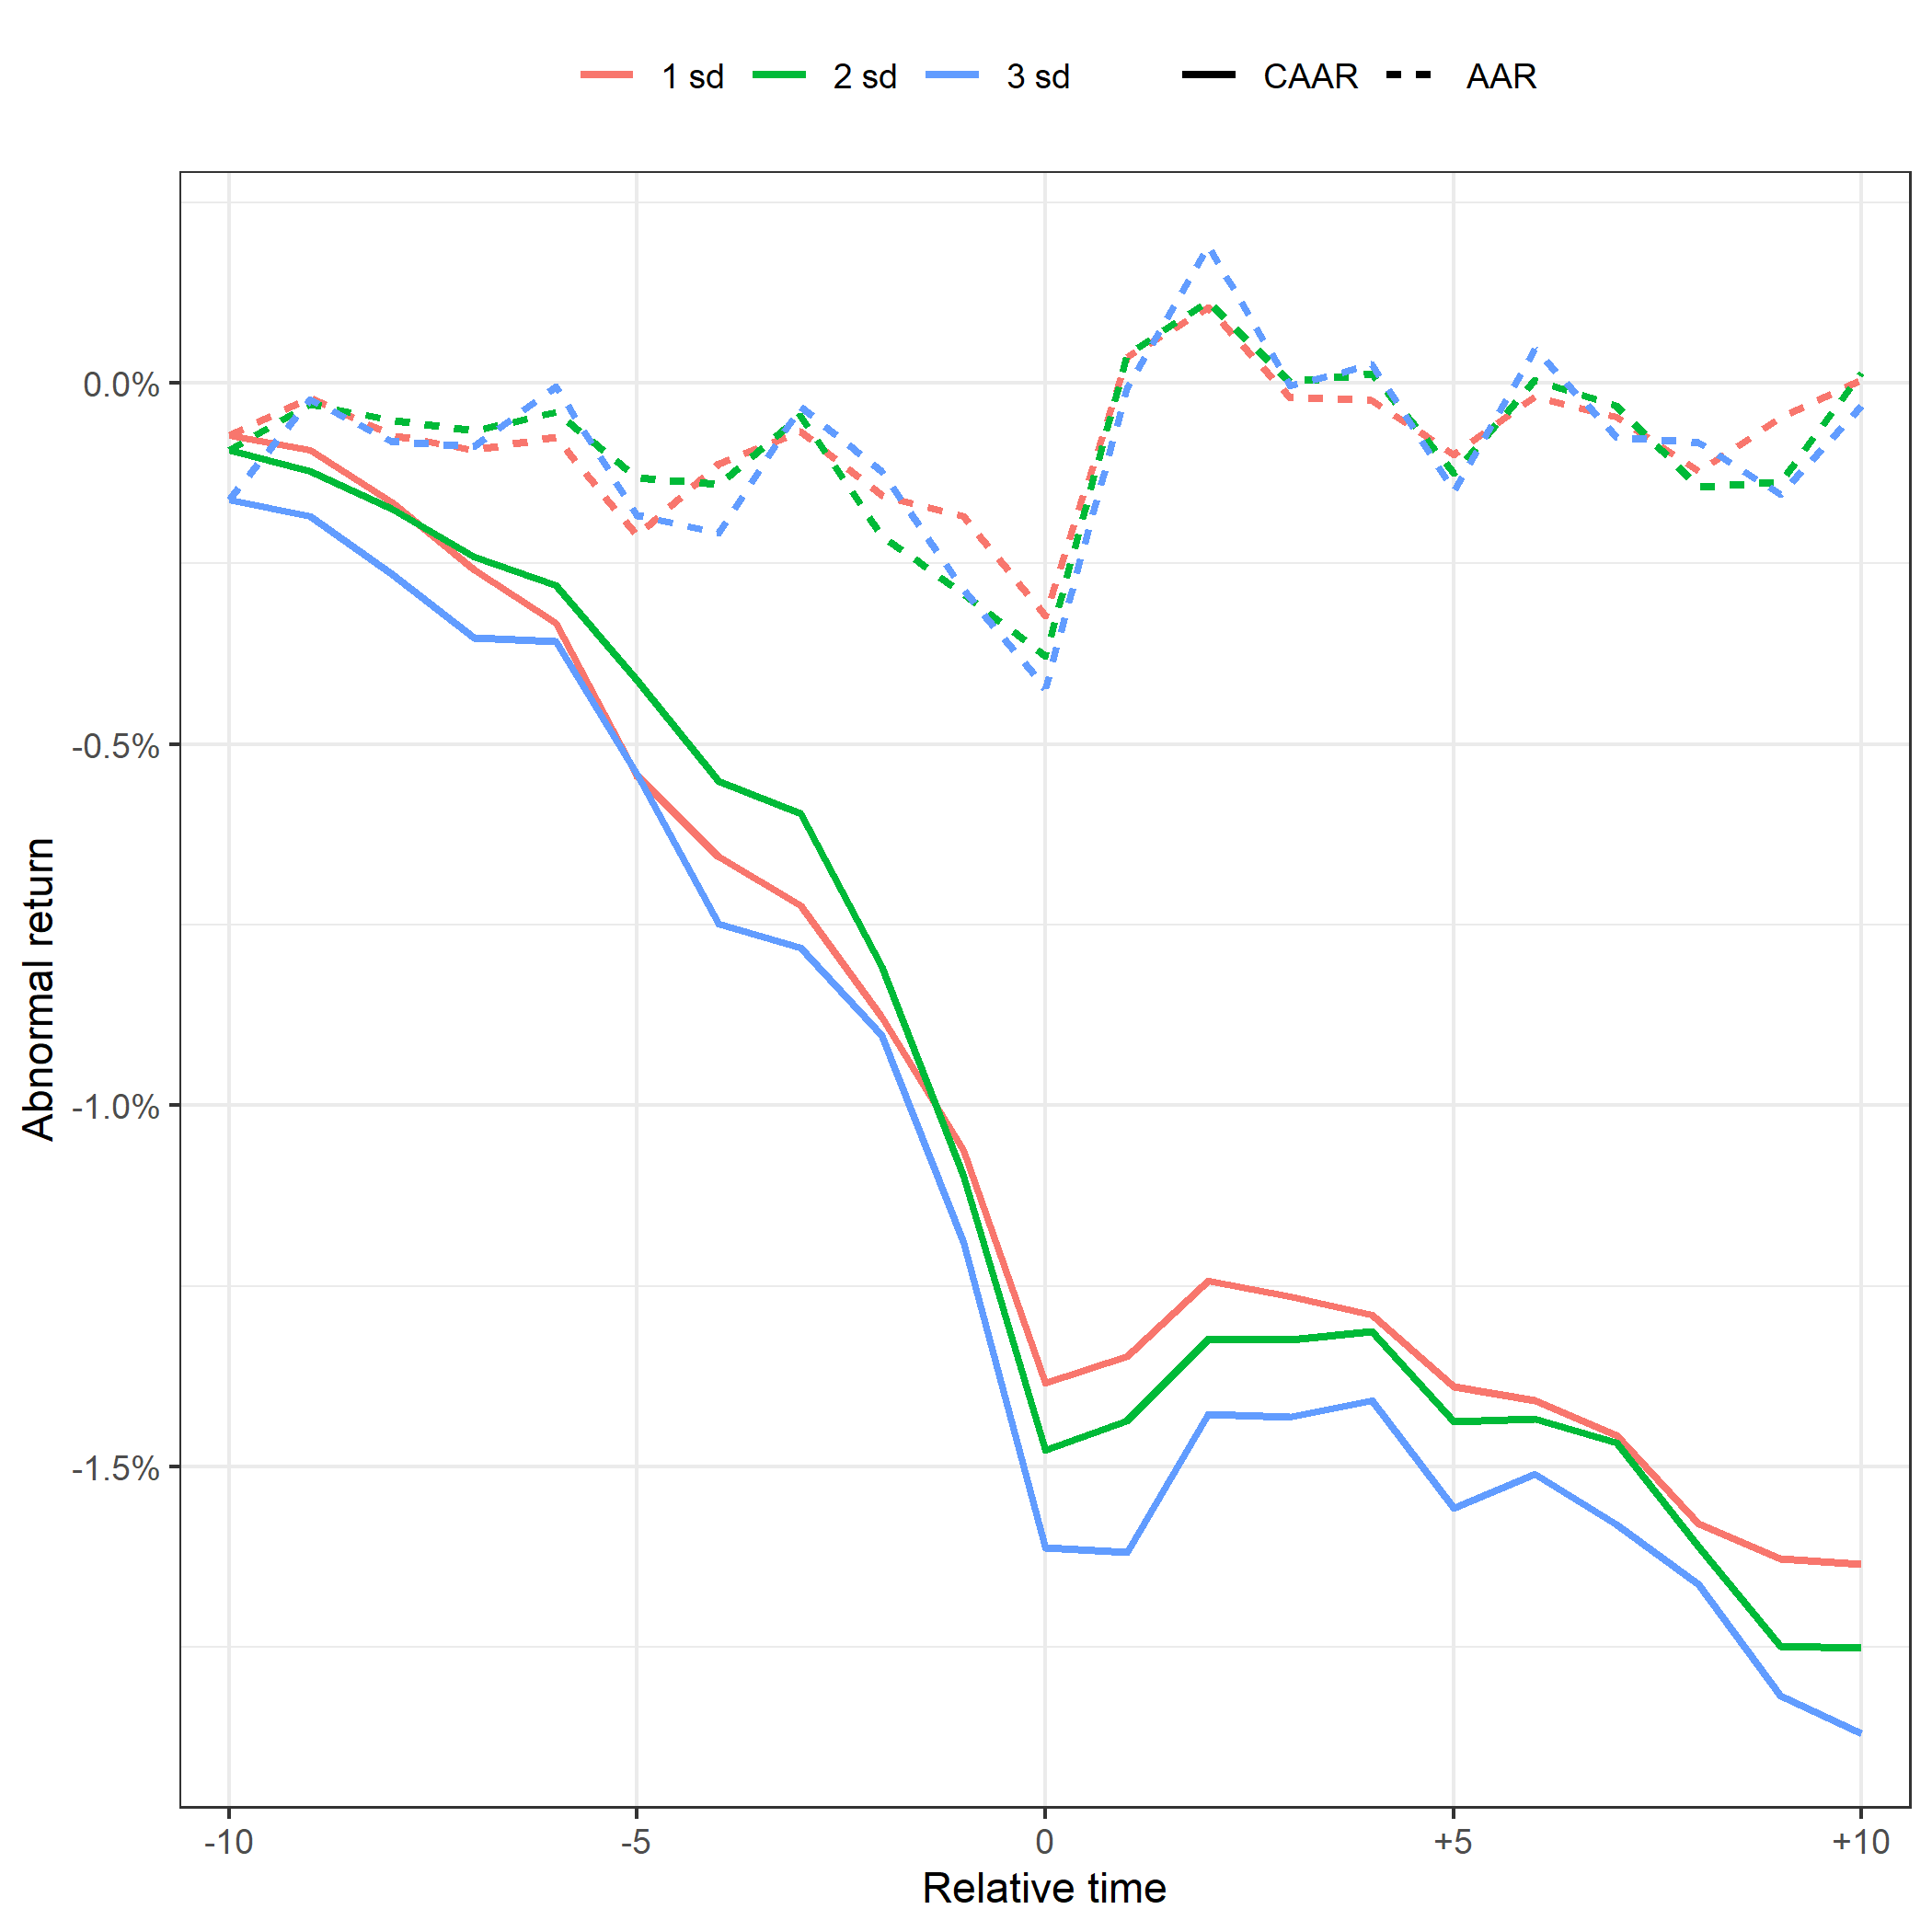
\includegraphics[scale=0.6]{Projekt/1.Figures analysis/ST_negative_sensitivity.png}
     \caption*{\footnotesize The figure illustrates the AAR and CAAR around the event date (t = 0) of negative news. The various colors represent the event identification rule of 1, 2, or 3 standard errors. The groups have, respectively, 1618, 957, and 683 events for 1,2, and 3 standard deviations}
    \label{fig:ST_neg_sensitivity}
\end{figure} 

The two new models, based on negative events, are compared to the original outcome (1sd) in figure \ref{fig:ST_neg_sensitivity}. The AAR is presented in dotted lines and the CAAR in solid lines for thresholds applying 2 sd (green) and 3 sd (blue). For simplicity, I have skipped the confidence intervals along with the bars. The similarities of the AAR and CAAR imply that the results are robust to changes in the event specification. Enforcing a stronger sd requirement leads to greater instantaneous impact on AAR on the event date. Moreover, a slight increase in CAAR signify a more severe reaction over the full window. 

\subsection{Market model: value vs. equal weights} \label{sec: sens_st_weights}

A portfolio of stocks needs to incorporate a weighted procedure in order to determine the relative impact the individual constituents should on portfolio performance. Figure \ref{fig:ST_neg_sensitivity_weight} compares the performance of applying value and equal weights to the an identical sample of firms experiencing negative events. 

\begin{figure}[H]
    \centering
    \caption{Negative news: Value vs. Equal weights}
    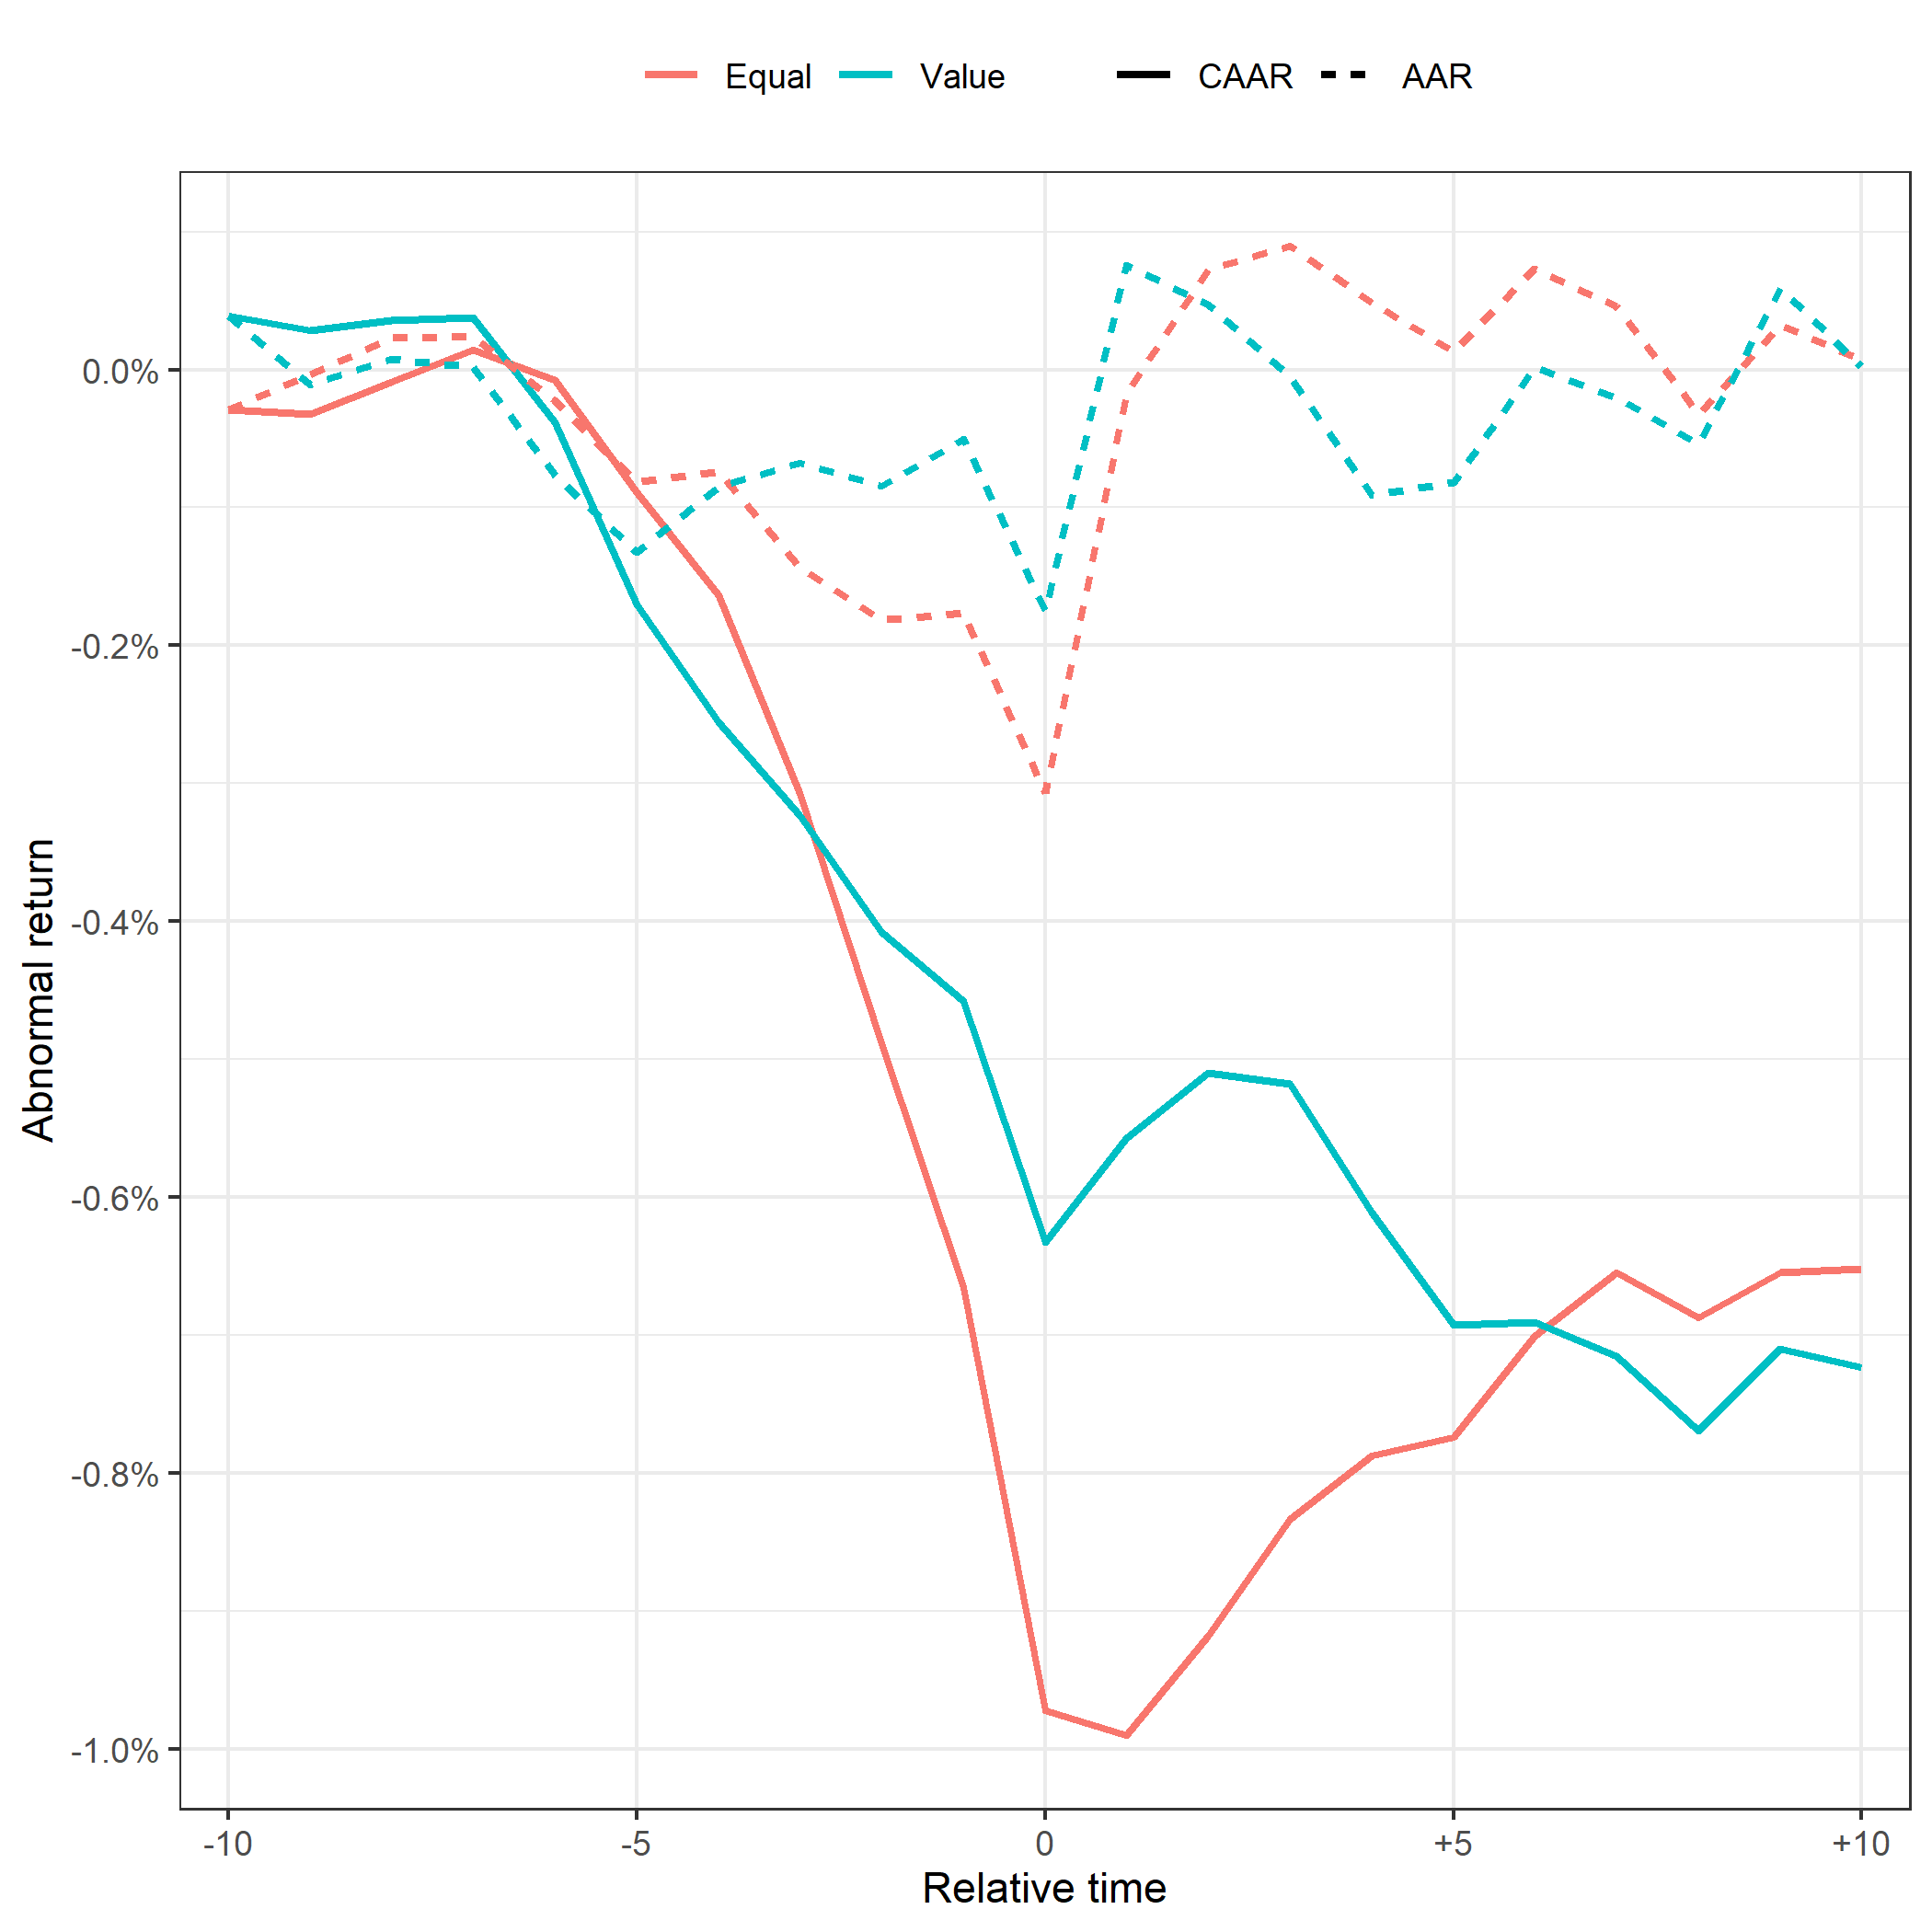
\includegraphics[scale=0.6]{Projekt/1.Figures analysis/ST_negative_sensitivity_weight.png}
     \caption*{\footnotesize The figure illustrates the average abnormal return (AAR) and cumulative AAR (CAAR) around the event date (t = 0) of negative news. The blue lines are returns calculated from an equally weighted portfolio, while the red lines are based on market capitalization weights.}
    \label{fig:ST_neg_sensitivity_weight}
\end{figure} 


The equal weighted portfolio returns validate the ordinary results, as the CAAR only diverge slightly and appear significant on the equal levels. While the portfolio AARs apparently follow each other to some extent, the development in CAAR is more adverse using equal weights relative to value weights. Applying equal weights inevitably allocates more weight to smaller stocks, which apparently contribute to less severe investor reactions. After the event has occurred the portfolio CAARs diverge, however as the AAR is statistically indifferent to zero in all days, the reactions are simply assumed to be minor estimation errors.    

\subsection{Calendar Time Portfolio: Portfolio weights}

Table \ref{tab: FF5_sensitivity} reports the alphas, t-values and significance levels of equally weighted portfolios along with the results from changing the threshold requirements. Besides the weights, the portfolio construction is identical to that from the empirical results in section \ref{sec: long_term_portfolio}. 

Altering the portfolio weights from value to equal clearly indicate a discrepancy from measurement with the latter generating higher absolute alpha values. The value weighted portfolio with T = 1 generated abnormal returns of -0.84\%, while the equivalent portfolio with equal weights ends up at -0.96\% significant on the $1\%$ level.   

The results are in contrast with the short term sensitivity analysis on portfolio weights, where the equal weighted portfolio generated lower abnormal returns. Again, the increased allocation toward smaller stocks seems to have an influential impact on the long run, however in the opposite direction relative to the short term. Applying holding periods of T = 8 and 12 months generate significant alpha as well indicating that smaller stocks are penalized over a longer time horizon than relatively larger ones.   

The abnormal returns of the equal weighted portfolios confirm the negative association between negative events and abnormal returns and to some degree the magnitude of the value weighted portfolio returns.

\setlength{\tabcolsep}{15pt}
\begin{table}[H]
\small
\centering
\caption{FF-5 alpha with equal weights and edit event rule } 
\makebox[\textwidth][c] {
\begin{tabular}{ccccccc}
\hline \hline \\ 
& &  Equal & & \multicolumn{2}{c}{ Value  } & \\ \cline{3-3} \cline{5-6}
  & & (1 SD) & & 2 SD  &  3 SD  & \\   
 & & & T = 1  & & \\ \cline{2-6}
 &  Alpha & $-0.96^{***}$  & &  -0.47  & -0.78  &  \\ 
 & t-value &  -3.80 &  & -0.97  & -1.63 & \\
 & &   & T = 4  & \\ \cline{2-6}
 & Alpha & $-0.70^{***}$ &  & $-0.45$ &  -0.27 & \\
 & t-value & -3.93 & & -1.58  & -1.04  & \\
 & &  & T = 8  & \\ \cline{2-6}
 & Alpha  & $-0.64^{***}$ & & -0.14 & -0.12 &  \\
 & t-value  & -4.20 & & -0.89 & -0.68 & \\
& &  & T = 12  & \\ \cline{2-6}
 & Alpha  & $-0.49^{***}$ &  & -0.16 & -0.17 &  \\
 & t-value & -3.71 & & -1.16 &  -0.97  & \\ \hline \hline
 \multicolumn{7}{l}{ \footnotesize $^* \; p\; <\; 0.1$, $ ^{**} \; p\; <\; 0.05$, $ ^{***} \; p\; <\; 0.01$  } \\
 \multicolumn{7}{p{12cm}}{ \footnotesize Alpha is the WLS-regression intercept (in \%) of the Fama-French 5-factor model, displayed along with the corresponding t-value. N is the average amount of firms included in the portfolio each month, and T is the portfolio holding period. The threshold for event firms to be included in the portfolio is either 1,2 or 3 "SD" (standard deviations) larger than the mean.} \\ 
 \hline
\end{tabular}
}
\label{tab: FF5_sensitivity}
\end{table}

\subsection{Calendar Time Portfolio: Thresholds}

Altering the threshold requirements from one to two and three standard leads to varying outcomes. For holding periods of one month, the alphas decrease and become insignificant from tightening the threshold, however the portfolio with three standard errors produce larger alphas than the one with two. With T = 4 the relation is reverse as the 2 standard deviation portfolio generates the largest alpha. Longer holding periods generate roughly equal abnormal returns across threshold values. As the portfolios are generating seemingly random outcomes, I reason that there is no relation between the event threshold and portfolio return on the long horizon. 


\subsection{New data}

\begin{figure}[H]
    \centering
    \caption{Negative news: Nasdaq Global}
    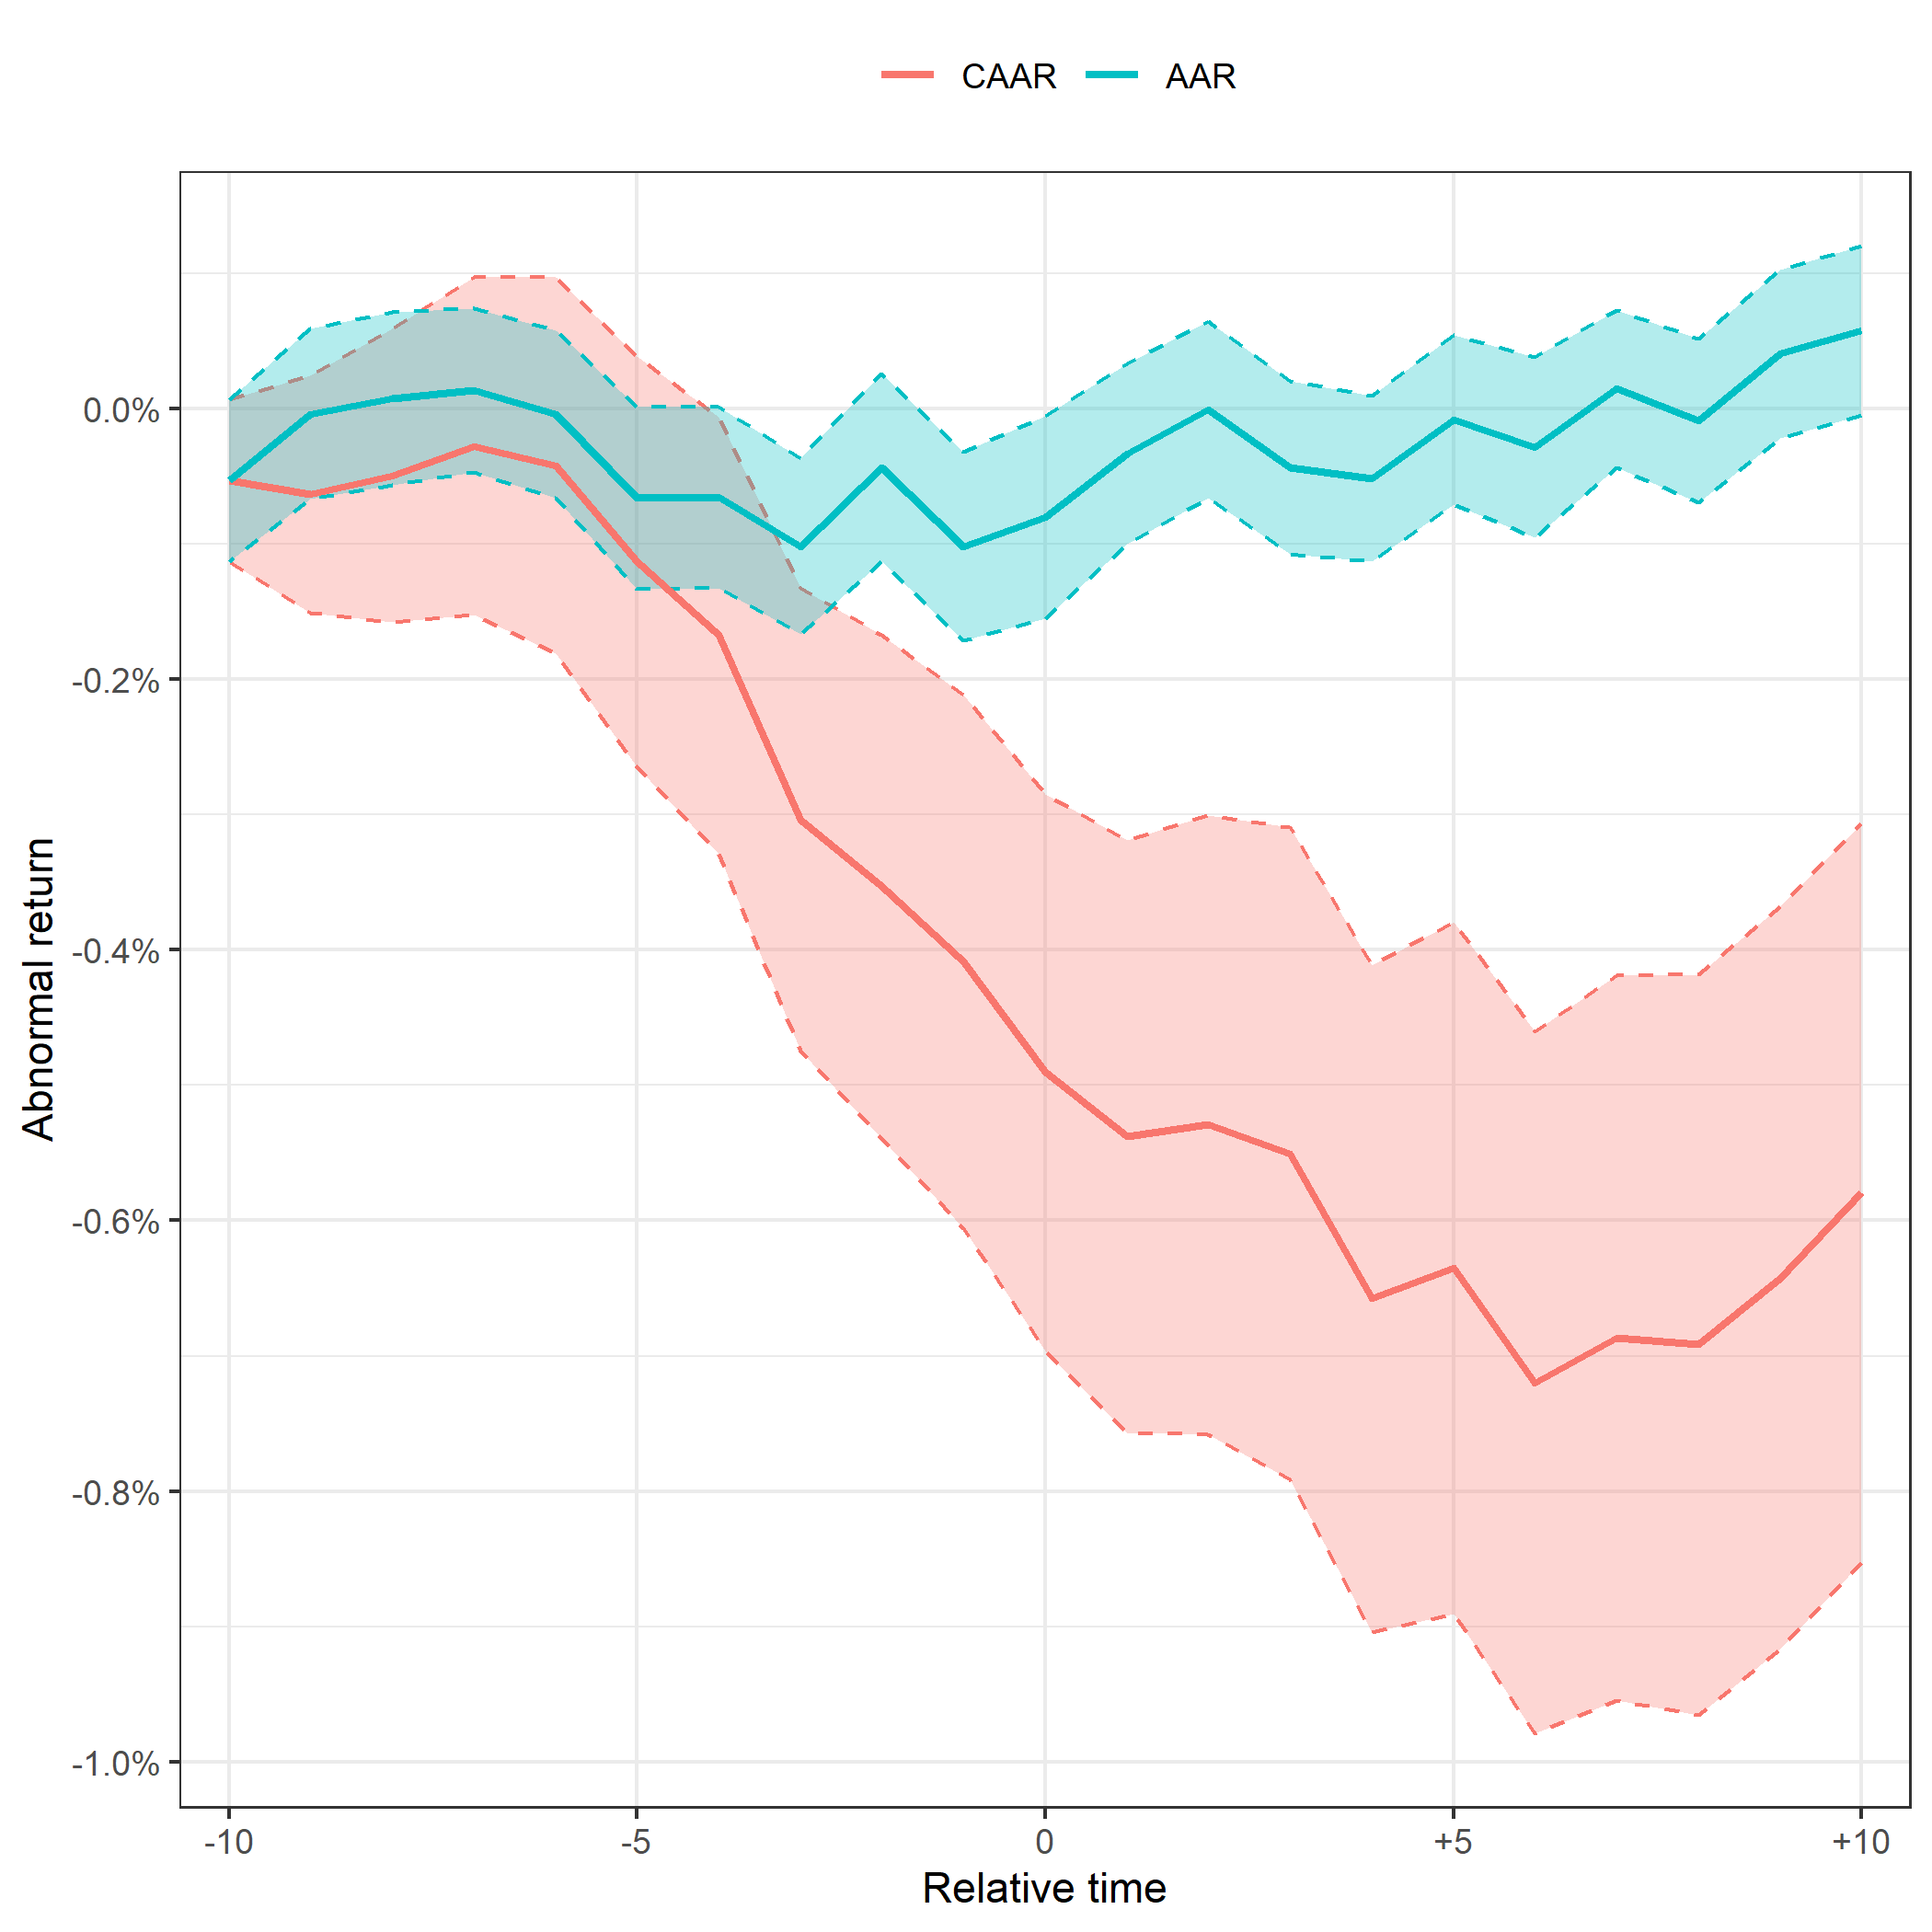
\includegraphics[scale=0.6]{Projekt/1.Figures analysis/ST_negative_all_CI_nasdaq.png}
     \caption*{\footnotesize The figure illustrates the average abnormal return (AAR) and cumulative AAR (CAAR) around the event date (t = 0) of negative news. The blue lines are returns calculated from an equally weighted portfolio, while the red lines are based on market capitalization weights.}
    \label{fig:ST_neg_sensitivity_weight}
\end{figure} 